% !TeX spellcheck = en_US
\section{How does the decline of HPV changes if the percentage of MSMs increases significantly?}
As we mentioned before, the data used in this work is a little bit old and the sexual behavior of the people has experimented changes in the last years. Thus, it would be interesting to perform some simulations adapting properly the model parameters. Here, we propose an increasing in the percentage of men who have sex with men (MSM). This simulation can be also considered as a sensitivity analysis to support the robustness of the present study with respect to the variation of the percentage of MSM.

In our proposal we have assumed that the percentage of MSM in the population is $3.88\%$. This value is provided by \cite{INE}. However, this survey was published in 2003. Then, here, we are going to increase the percentage of MSM from $3.88\%$ until $10\%$. Only girls are vaccinated with a $70\%$ coverage (Spanish current program). 

\begin{figure}[!]
	\centering
	\begin{tabular}{cc}
		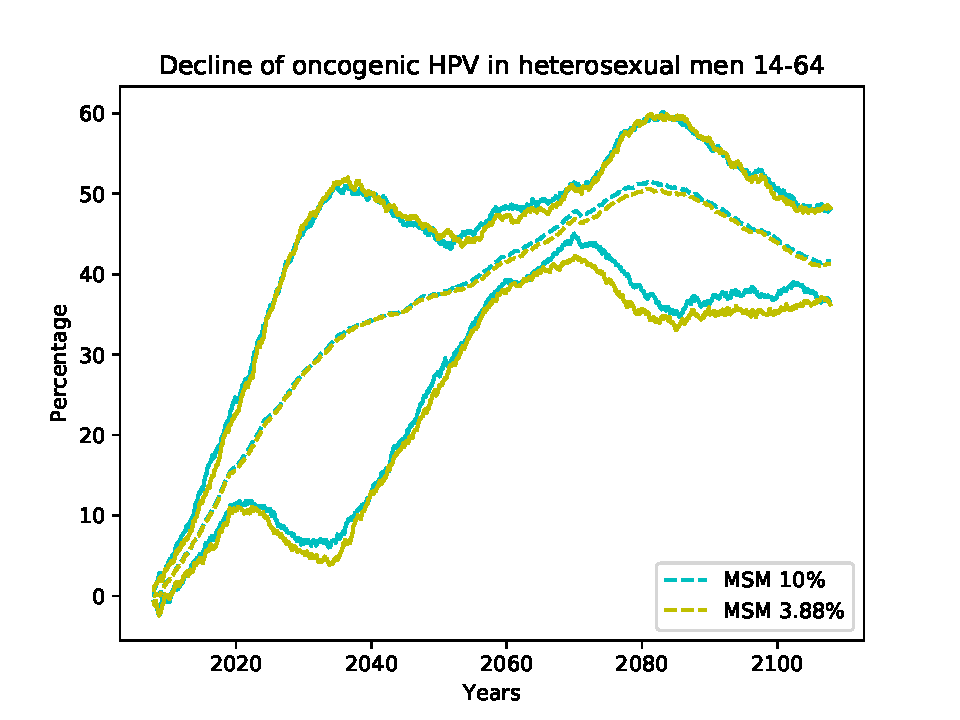
\includegraphics[width=0.5\linewidth]{IMGs/13.-Aumento_MSM/onco_hom_hetero.pdf}	& 
		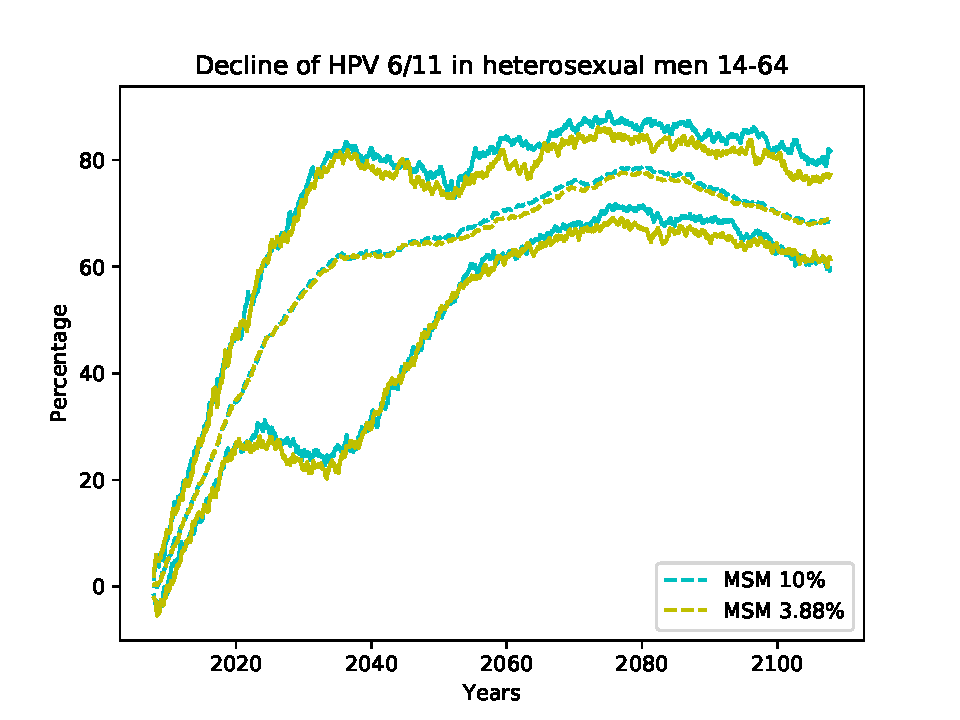
\includegraphics[width=0.5\linewidth]{IMGs/13.-Aumento_MSM/verr_hom_hetero.pdf}  \\ 
		Decline oncogenic HPV hetero men	& Decline HPV 6/11 hetero men \\ 
		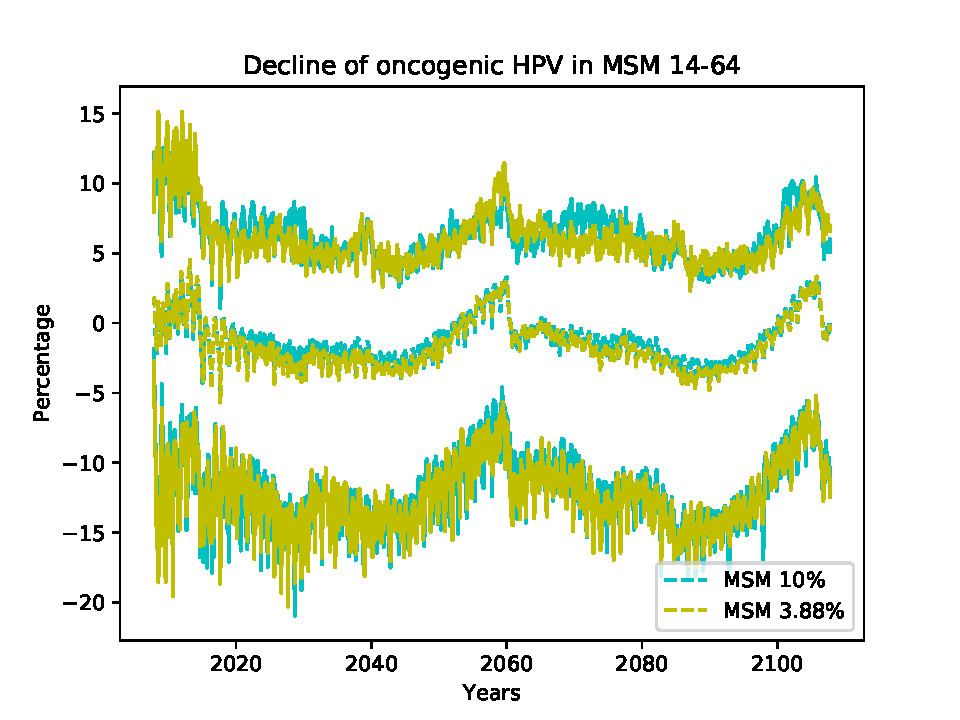
\includegraphics[width=0.5\linewidth]{IMGs/13.-Aumento_MSM/onco_MSM.pdf}	& 
		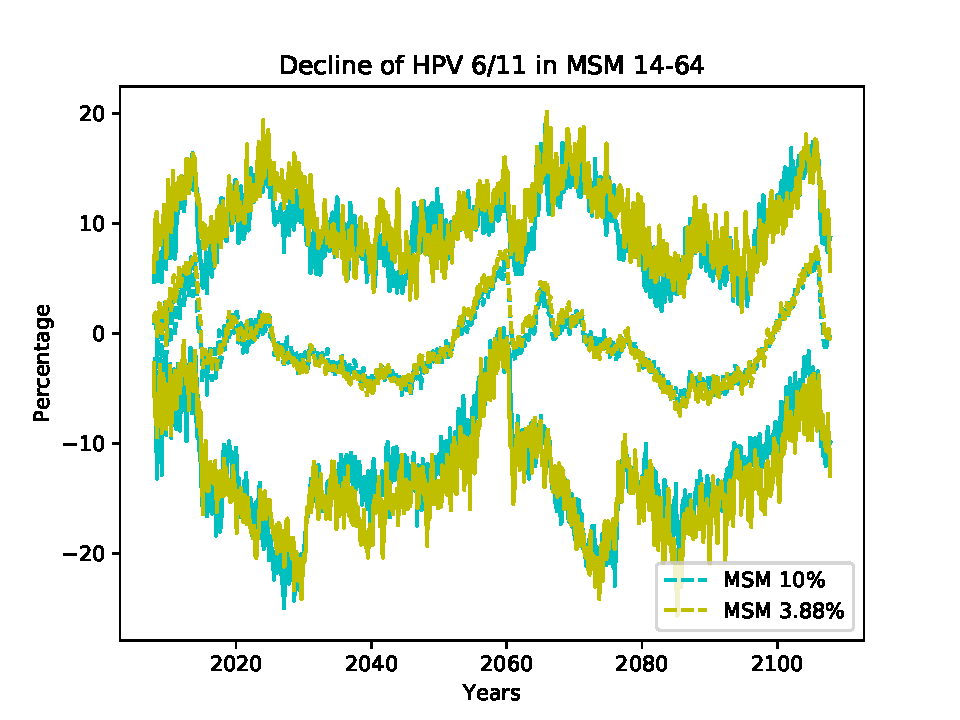
\includegraphics[width=0.5\linewidth]{IMGs/13.-Aumento_MSM/verr_MSM.pdf}  \\ 
		Decline oncogenic HPV MSM	& Decline HPV 6/11 MSM \\ 
		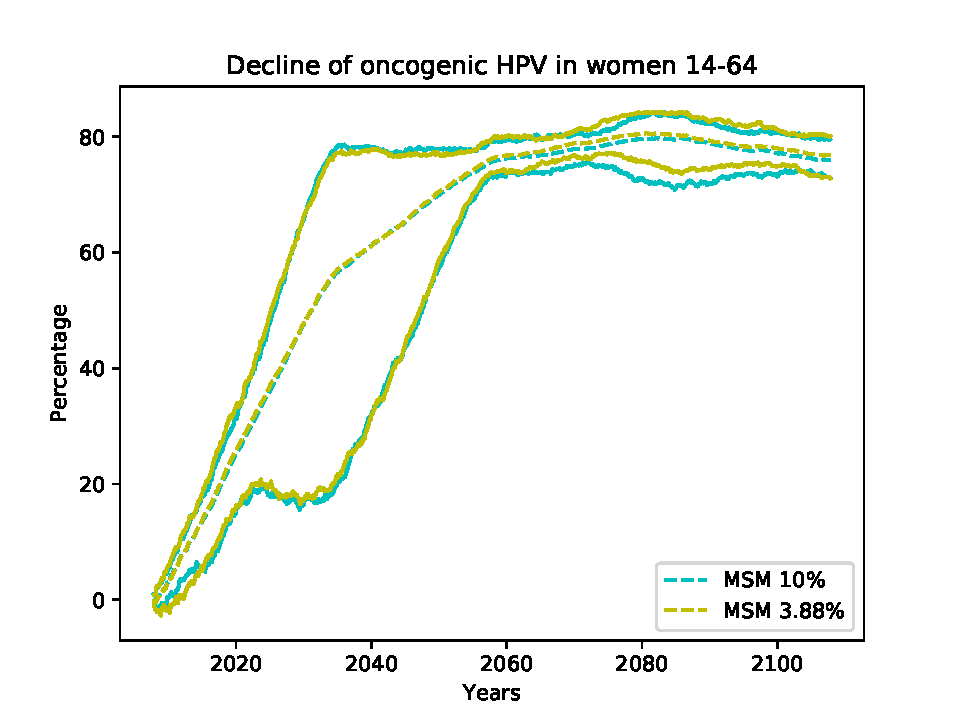
\includegraphics[width=0.5\linewidth]{IMGs/13.-Aumento_MSM/onco_muj.pdf}	& 
		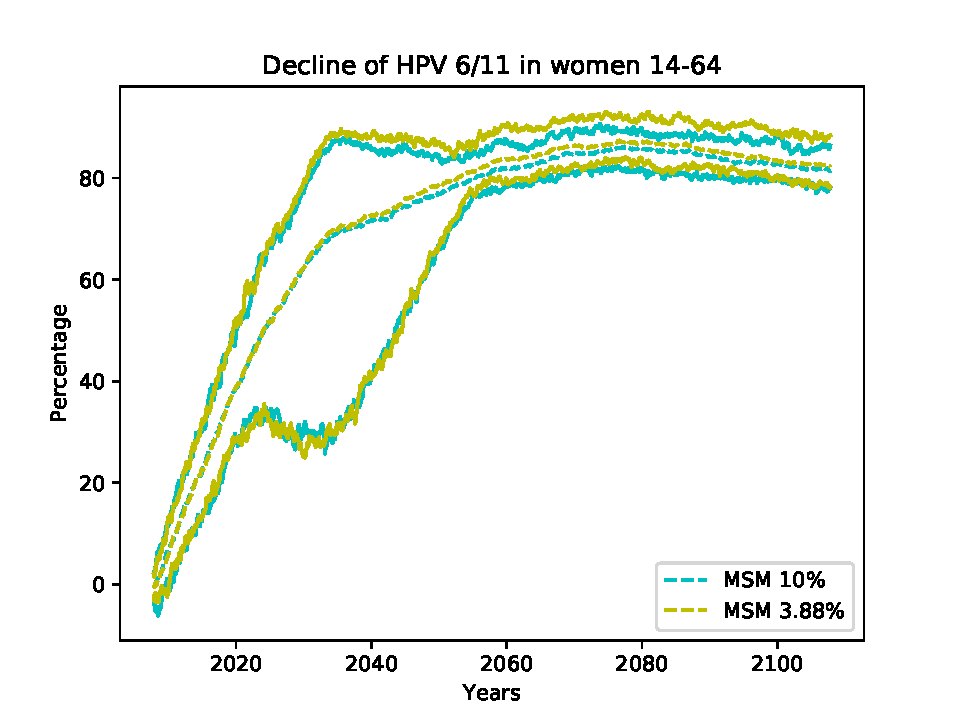
\includegraphics[width=0.5\linewidth]{IMGs/13.-Aumento_MSM/verr_muj.pdf}  \\ 
		Decline oncogenic HPV women	& Decline HPV 6/11 women \\ 
	\end{tabular} 
	\caption{Comparative of the decline of HPV in case the number of MSM increases from $3.88\%$ until $10\%$. In the current vaccination scenario (vaccinating only girls with a coverage of $70\%$, there are not significant declines in heterosexual men, MSM and women. The graphs corresponding to heterosexual men show a higher decline as those considering both heterosexual and homosexual men.}
	\label{fig:compara_MSM}
\end{figure}

As we can see in Figure \ref{fig:compara_MSM}, the decline hardly changes in heterosexual men, MSM and women. This means that the increase of MSM only affects themselves, because they do not have herd immunity effect.

Furthermore, Figure \ref{fig:compara_MSM} shows the decline in heterosexual men. Note that the levels of decline for HPV 6/11 achieves more than $70\%$ in the long-run vaccinating girls with a coverage of $70\%$, meanwhile the girls achieves a decline higher than $80\%$. In the case of oncogenic HPV, the decline is not so high and it is more uncertain, achieving around $50\%$ in heterosexual men and around $80\%$ in women. With this comment we may have an idea about the protection provided by GARDASIL and GARDASIL9 in the women and heterosexual men network, in the long-run.